\chapter{Adding}

In this model, we found 2 flavors of period-adding structures.
The first one is period adding in between the chains of the same period.
The other is period adding near ``type B'' period regions.

\section{Adding in Between Chains of the Same Period}

\Cref{fig:minrep.adding1.overview} shows both the periods of the model initially, as described in the previous chapter (\Cref{chap:minrep}), as well as the model with period-adding structures.
For \Cref{fig:minrep.adding1.overview.adding}, only the values of the fixed parameters $a_L = 1, b_L = 0.5$ are changed.
Initially, the values for these parameters were $a_L = 4, b_L = -0.5$.
The only other fixed parameter $B$ stays the same and the parameter ranges of $p_x$ and $p_y$ were adjusted slightly.
That means, that the shape of the function only changed on the branches $f_{\A}$ and $f_{\C}$.

When comparing both figures, we can see that there are no ``type B'' period regions in \Cref{fig:minrep.adding1.overview.adding}, the period-adding situation.
Instead, it looks like the ``type A'' period regions of the same period overlap now.
Also, the regions of higher periods in between the chains are new, these are the period-adding regions.
At the points, where these regions make a turn, there are period regions of even higher periods.
The meaning of these is explored in a later section, the next section will focus on the disappearance of the ``type B'' parameter regions.

\begin{figure}
    \centering
    \subfloat[Initial situation]{
        \includegraphics[width=.5 \textwidth]{62_MinimalRepr_Adding/2D_Period_4/result.png}
    }
    \subfloat[Period-adding]{
        \includegraphics[width=.5 \textwidth]{62_MinimalRepr_Adding/2D_Period_1/result.png}
        \label{fig:minrep.adding1.overview.adding}
    }
    \caption{Overview of period-adding structures in between chains of the same period}
    \label{fig:minrep.adding1.overview}
\end{figure}

\subsection{Disappearance of ``Type B'' Parameter Regions}

\Cref{fig:minrep.path.to.disappearance} shows diagrams depicting the borders of parameter regions of specific stable cycles.
The lower left corner of the diagrams is always in the period region with the stable cycle $\Cycle{\A^7\B^3\C^7\D^3}$, the cycles in the upper left ($\Cycle{\A^6\B^3\C^6\D^3}$), upper right ($\Cycle{\A^6\B^4\C^6\D^4}$), lower right ($\Cycle{\A^7\B^4\C^7\D^4}$), and middle ($\Cycle{\A^7\B^3\C^6\D^4}$ and $\Cycle{\A^6\B^4\C^7\D^3}$) follow.
The diagrams show the evolution of the ``type B'' parameter region along a line in the parameter space from $a_L = 4, b_L = -0.5$ to $a_L = 1, b_L = 0.5$.
This line is given by the equation $a_L = \frac{5}{2} - 3 \cdot b_L$.

The first figure, \Cref{fig:minrep.path.to.disappearance.0}, shows the parameter regions at the initial situation.
As described in \Cref{sec:minrep.coex}, ``type A'' parameter regions overlap with ``type A'' parameter regions of different periods and with ``type B'' parameter regions.
In \Cref{fig:minrep.path.to.disappearance.1}, this overlap still exists between the lower and upper left parameter regions, as well as the lower right parameter region with each other.
Also the upper left and upper right parameter region overlap.
But the boundaries of the ``type B'' parameter region are almost identical to the boundaries of the neighboring ``type A'' parameter regions.
The upper and lower right parameter regions no longer overlap, instead, there is space in between where the period-adding of the two cycles of each parameter region happens.


\begin{figure}
    \centering
    \subfloat[$a_L = 4, b_L = -0.5$]{
        \includegraphics[width=.3 \textwidth]{62_MinimalRepr_Adding/2D_Regions_4/Manual/result.png}
        \label{fig:minrep.path.to.disappearance.0}
    }
    \subfloat[$a_L = 2.4, b_L = -0.1$]{
        \includegraphics[width=.3 \textwidth]{62_MinimalRepr_Adding/2D_Regions_2.4/Manual/result.png}
        \label{fig:minrep.path.to.disappearance.1}
    }
    \subfloat[$a_L = 2.25, b_L = -0.0625$]{
        \includegraphics[width=.3 \textwidth]{62_MinimalRepr_Adding/2D_Regions_2.25/Manual/result.png}
    } \\
    \subfloat[$a_L = 2.225, b_L = -05625$]{
        \includegraphics[width=.3 \textwidth]{62_MinimalRepr_Adding/2D_Regions_2.225/Manual/result.png}
    }
    \subfloat[$a_L = 2.2, b_L = -0.05$]{
        \includegraphics[width=.3 \textwidth]{62_MinimalRepr_Adding/2D_Regions_2.5/Manual/result.png}
    }
    \caption{\todo{caption}}
    \label{fig:minrep.path.to.disappearance}
\end{figure}
